% --- PRÉAMBULE ---
\documentclass[a4paper, 11pt]{article}

% --- Paquets pour le français et l'encodage ---
\usepackage[utf8]{inputenc}
\usepackage[T1]{fontenc}
\usepackage[french]{babel}

% --- PAQUETS CORRIGÉS / AJOUTÉS ---
\usepackage{xcolor} % Pour définir et utiliser des couleurs
\usepackage{colortbl} % Pour la commande \rowcolor dans les tableaux
\usepackage{tabularx} % Pour l'environnement tabularx
\usepackage{enumitem} % Pour personnaliser les listes (label=$\circ$ et label=$\bullet$)
\usepackage{array}    % Pour améliorer les tableaux

\usepackage{geometry}
\geometry{a4paper, margin=2.5cm} % Marges
\usepackage{graphicx} % Pour inclure des images
\usepackage{hyperref} % Pour les liens cliquables (ex: table des matières)
\hypersetup{
    colorlinks=true,
    linkcolor=black,
    urlcolor=blue,
}
\usepackage{amsmath} % Pour les formules mathématiques
\usepackage{appendix}
\usepackage{pdfpages}
\usepackage{makecell}

% --- Coloration / code ---
\usepackage{listings}
\lstdefinelanguage{Chips}{
  morekeywords={logical,physical,object,system,init,then,spread,collect,as,with,implementation,input,stop,among,ctx,using,actuator,sensor},
  sensitive=true,
  morecomment=[l]{//},
  morestring=[b]"
}
\lstset{
  basicstyle=\ttfamily\small,
  keywordstyle=\color{blue}\bfseries,
  commentstyle=\color{gray},
  stringstyle=\color{red!60!black},
  showstringspaces=false,
  columns=fullflexible,
  frame=single,
  breaklines=true
}
\newcommand{\prog}[1]{\texttt{#1}}

% --- DÉBUT DU DOCUMENT ---
\begin{document}


\begin{titlepage}
  \begin{center}
    
\begin{figure}[ht]
    \centering
    \begin{minipage}{0.45\textwidth}
        \centering
        
\includegraphics[height=22mm]{logo-UFRST-DeptInfo.png}
    \end{minipage}
    \hfill % Petit espacement entre les deux blocs
    \begin{minipage}{0.45\textwidth}
        \centering
        
\includegraphics[height=22mm]{LOGO_UMLP.png}
    \end{minipage}
\end{figure}
    
   \vspace{1cm}
% \marginpar{OlgaK : les logos UMLP et UFR ST doivent être ensemble en haut, en plus petit}   

         % --- Université et Master ---
  {\large\scshape Université Marie \& Louis Pasteur \\ Département informatique\par} % \scshape pour petites majuscules
  \vspace{0.5em} % Petit espace
  {\large Master 2 en Ingénierie Système et Logiciel\par} % Taille de police standard pour le master
    
        \vspace{1.2cm}
    \centerline{\hbox to 13cm{\hrulefill}}
    \vspace{0.3cm}
    {\sc \Large  \uppercase{{
        Implantation d'un parseur et ajout d'un jeu d'instructions pour le langage CHIPS
    }}}
    \centerline{\hbox to 13cm{\hrulefill}}
    
    \vspace{1.2cm}
    {\sc \Large {DOLARD ANTON} \\ [0.5 cm]
    \sc \Large {FOCHEUX VITAL} \\ [0.5 cm]
    \sc \Large {GAUTHIER JULIEN}\\ [0.5 cm]
    \sc \Large {TUTRICES :} \\ [0.5 cm]
    \sc \Large {GALLONE ANNA} \\ [0.5 cm]
    \sc \Large {KOUCHNARENKO OLGA}\\ [0.5 cm]
    }
    \vspace{1.5cm}

    \begin{figure}[h]
		\centering
		
\includegraphics[width=0.48\textwidth]{CHIPS.png}
    \end{figure}
    
    \vspace{0.5cm}
    

    
    \hbox to \textwidth{\hrulefill}
    \vspace{0.2cm}
    {\sc  RAPPORT DE PROJET DE MASTER 2 INGÉNIERIE SYSTÈME ET LOGICIEL - ANNÉE 2025/2026}
    
  \end{center}
\end{titlepage}



\thispagestyle{empty}
\clearpage

\newpage

\section*{Remerciements}

Nous tenons à remercier nos tutrices de projet, Mme \textsc{KOUCHNARENKO} et Mme \textsc{GALLONE} 
qui ont su nous conseiller tout au long de ce projet.

\newpage

\newpage
\tableofcontents % Crée la table des matières
\newpage

\newpage
\setcounter{page}{1} % Commence la numérotation des pages à 1 ici

\section{Introduction}

Dans le cadre de la modélisation de systèmes distribués en vue de leur simulation et implantation un langage est en cours de développement au DISC\footnote{Département Informatique de Système Complexe}. Ce langage, CHIPS\footnote{Control of Hierarchical Interconnected Programmable Systems}, vise à représenter les applications distibuées sous la forme de deux graphes : \textbf{un graphe fonctionnel} représentant les algorithmes par ses nœuds et des flux de données par ses arrêtes, et \textbf{un graphe de dépendance physique} utilisant les mêmes nœuds et ajoutant un second type d'arrêtes pour signifier le rattachement des algorithmes à leur support physique. \\

Lors de ce rapport, nous allons détailler les différents aspects conceptuels et techniques de ce projet. Nous commencerons par présenter les besoins et objectifs du projet. Ensuite, nous détaillerons les algorithmes et les technologies utilisés et mis en place pour mettre en œuvre ce projet, comme le lexing et le parsing de la grammaire mais aussi la sérialisation vers le langage XMI\footnote{XML Metadata Interchange}. Suivront des explications pour gérer les erreurs au moyen de génération de tests ainsi que du parcours de l'AST\footnote{Abstract Syntax Tree}. Nous évoquerons une partie sur la gestion du projet et ce qui a été mis en œuvre. Enfin nous pourrons conclure sur ce projet sur un bilan technique où nous évoquerons ce qui a pu être réalisé mais aussi ce qui aurait pu être réalisé, et aussi un bilan personnel.

\section{Besoins et objectifs du projet}

\subsection{Contexte}

\subsection{Motivations}

\subsection{Objectifs}

Parmi les objectifs, il y a ceux qui avaient été demandés comme :
\begin{itemize}
    \item Compléter un parseur C++/Yacc/Bison.
    \item Intégrer de nouvelles constructions syntaxiques représentant les fonctions collectives\footnote{Ces fonctions sont \prog{collect} et \prog{spread}} qui n'étaient pas encore supportées par le langage.
    \item La gestion des erreurs syntaxiques et sémantiques.
\end{itemize} 

Mais certains objectifs ont pu être ajoutés au cours du projet que cela soit par nos tutrices ou bien par nous comme :
\begin{itemize}
    \item La sérialisation de l'AST vers le langage XMI.
    \item Un modèle GBT\footnote{Grammar Based Testing} afin de créer des tests d'acceptation pour le langage.
\end{itemize}

\section{Algorithmes et technologies}

\subsection{Lexing et parsing de la grammaire}

\subsubsection{Lexing}

Afin d'avoir une grammaire utilisable il faut qu'auparavant on puisse créer des jetons, des symboles terminaux. Pour cela, nous utilisons l'outil libre \prog{Flex} qui est un analyseur lexical. Il va nous permettre grâce à des expressions régulières de déterminer certains jetons comme :
\begin{itemize}
    \item \prog{DIGIT [0-9]} $\longrightarrow$ représentation d'un chiffre
    \item \prog{IDENT [a-zA-Z][a-zA-Z0-9\_]*} $\longrightarrow$ représentation des identifiants
\end{itemize}

Ceux-ci nous permettent par la suite de faire la représentation des littéraux (cf: \nameref{fig:jetons_literal}), des opérateurs binaires et unaires (cf: \nameref{fig:jetons_binaires_unaires}), des types de données et fonctions (cf: \nameref{fig:jetons_type_donnees} et \nameref{fig:jetons_type_func}), des littéraux qu'on peut retrouver dans d'autres langages comme C (cf: \nameref{fig:jetons_C}) et enfin les littéraux qui sont spécifiques à CHIPS (cf: \nameref{lst:jetons}). \\

Une fois tous les jetons terminaux instanciés nous allons pouvoir nous en servir durant le parsing et la création de l'AST avec les règles de la grammaire que nous allons évoquer dans la partie suivante.

\subsubsection{Parsing}

Une fois tous les jetons terminaux définis, nous allons pouvoir écrire les règles du langage, c'est ce qui nous permet en parcourant la première règle d'atteindre des règles ``terminales''\footnote{C'est-à-dire qu'elle contient que des jetons terminaux ou bien les jetons non-terminaux sont soit vides soit un seul jeton terminal}. Pour cela, nous utilisons l'outil \prog{Yacc} qui est un outil de génération d'analyseurs syntaxiques en langage C. \\

Par exemple la règle pour définir une fonction physique (cf: \nameref{fig:grammar_physical}) où on va définir le nom de la règle, ici \prog{p\_function\_def}, et on va lui définir la suite de jetons qu'elle peut prendre, ici des jetons terminaux qui sont : 
\begin{itemize}
    \item \prog{PHYSICAL\_KW} $\longrightarrow$ qui correspond au jeton \prog{physical}
    \item \prog{IDENTIFIER} $\longrightarrow$ qui correspond au jeton pour les identifiants
    \item \prog{L\_PARENTH} $\longrightarrow$ qui correspond au jeton pour "("
    \item \prog{R\_PARENTH} $\longrightarrow$ qui correspond au jeton pour ")"
\end{itemize}

et des jetons non-terminaux qui sont :
\begin{itemize}
    \item \prog{pdf\_parameter\_list} $\longrightarrow$ qui correspond à la règle de la grammaire pour la liste des paramètres des fonctions physiques
    \item \prog{with\_section} $\longrightarrow$ qui correspond à la règle de la grammaire pour la section \prog{with}
    \item \prog{init\_section} $\longrightarrow$ qui correspond à la règle de la grammaire pour la section \prog{init}
    \item \prog{then\_section} $\longrightarrow$ qui correspond à la règle de la grammaire pour la section \prog{then}
    \item \prog{p\_named\_outputs} $\longrightarrow$ qui correspond à la règle de la grammaire pour les \prog{outputs} de la fonction physique
\end{itemize}

Après la définition de ou des règle(s), on va pouvoir créer le nœud de l'AST, où \verb|$$| correspond au nœud de l'AST sur lequel on va pouvoir potentiellement effectuer les fonctions de la classe. Le constructeur du nœud prend en paramètre \verb|$X| où \prog{X} correspond au numéro du jeton dans la règle. Le constructeur prend presque toujours en paramètre des jetons non-terminaux, seuls les jetons terminaux qui correspondent aux littéraux comme les identifiants, les booléens et les nombres peuvent être pris en paramètre. Dans cet exemple, l'identifiant de la fonction qui est un jeton terminal est pris en paramètre et il correspond à \verb|$2|. \\

Une fois le nœud instancié, nous allons pour certains nœuds utiliser leurs fonctions \verb|set_line(@$.begin.line)| et \verb|set_column(@$.begin.column)| qui correspondent respectivement à donner au nœud son numéro de ligne et son numéro de colonne.

\subsection{Sérialisation vers XMI}

La sérialisation vers XMI a pour objectif de transformer un programme CHIPS parsé en un modèle conforme au méta-modèle CHIPS (\prog{chips1.1.ecore} ou \prog{chips2.ecore}), afin de le manipuler ensuite dans l’écosystème Eclipse/EMF et de l’intégrer dans des chaînes de Model-Driven Engineering. Le flux global part d’un fichier \prog{.chips}, construit un AST, puis produit un fichier \prog{.xmi} dont les chemins sont stables et dont les références croisées sont résolues à l’aide d’une table des symboles.

Dans Eclipse, avec le plugin ATL (Atlas Transformation Language), un outil de transformation de Modèle à Modèle qui décrit les transformations à appliquer sous la forme de règles qui génèrent des éléments d'un modèle cible à partir d'éléments d'un modèle source. Ce fichier XMI peut ensuite servir de point d’entrée pour des transformations ATL vers d’autres méta-modèles, par exemple pour la génération de modèles de simulation ou d’implémentation. La validité syntaxique de XMI est vérifiée automatiquement par un script \prog{xmi\_validator.py}, ce qui nous permet de garantir que la génération est correcte sur un corpus d’exemples, même si certains nœuds de l’AST restent encore à traiter.

\subsubsection{Parcours de l'AST, pattern visiteur}

Le parcours de l’AST repose sur une classe \prog{ChipsToXmiVisitor} qui implémente l’interface \prog{chipsvisitor} et fournit une méthode de visite pour chaque type de nœud de l’AST CHIPS (définitions, \emph{statements} système, expressions, sections \prog{with}/\prog{init}/\prog{then}, etc.). Ce visiteur travaille toujours avec un chemin courant \prog{mcurrentastpath} qui encode la position d’un nœud dans l’arbre (par exemple \prog{preambledefinitions.0}, \prog{systemstatements.2}), ce qui permet ensuite de générer des chemins XMI stables pour toutes les déclarations et références.

Lors de la visite, le visiteur maintient deux structures centrales : une table des symboles \prog{msymboltable} qui associe un nom logique (variable, paramètre, \prog{channel}, fonction collective, etc.) à un couple \emph{(chemin XMI, type métier)}, et une table des définitions \prog{mdefinitionstable} qui enregistre les variables internes à chaque définition (\prog{with}/\prog{init}/\prog{then}). C’est sur ces tables que repose la résolution des références lors de la sérialisation : une variable déclarée avec un nom dans le code CHIPS (par exemple un \prog{channel} ou une variable contextuelle) est ensuite référencée par son chemin dans le XMI, ce qui oblige à retrouver, parfois depuis un autre endroit de l’AST, la bonne instance et à distinguer la variable elle-même de son contenu ou de sa déclaration.

Concrètement, chaque visite de nœud de déclaration enregistre son symbole : par exemple, un \prog{objectDefinitionNode}, un \prog{logicalFunctionDefinitionNode} ou un \newline \prog{physicalFunctionDefinitionNode} ajoute l’objet ou la fonction à la table des symboles avec un chemin de la forme \prog{preambledefinitions.X} et remplit la table des définitions avec les variables locales déclarées dans les sections \prog{with}, \prog{init}, \prog{then} et les paramètres de \emph{dataflow}. Les nœuds système comme \prog{functionnalBlockInstanciationNode}, \prog{implementsNode}, \prog{linkNode} ou \prog{pluggingNode} consultent ensuite ces tables pour retrouver le chemin précis des instances et des paramètres, afin d’écrire la bonne combinaison de \prog{xsitype}, de \prog{variable} et d’index dans le XMI (y compris pour des cas difficiles comme les mappings \prog{having} qui doivent parfois pointer vers la déclaration plutôt que vers la variable interne).

Une autre difficulté importante (détaillée en section~\ref{sec:problems-xmi}) a été de mapper correctement les sections du code CHIPS (\prog{preambles}, \prog{with}, \prog{init}, \prog{then}, opérations collectives, \emph{statements} système) vers les sections attendues du XMI, en respectant à la fois la structure du méta-modèle et les chemins utilisés par les fichiers de référence. Le visiteur encapsule cette logique dans des helpers qui détectent la « famille » d’un \emph{statement} (system, node, collective, implementation) et construisent les bons préfixes de type (par exemple \prog{chips.statements.system}, \newline \prog{chips.statements.collective}), ce qui permet de garder une correspondance claire entre l’AST et la hiérarchie XMI.

\paragraph{Exemple concret CHIPS \texorpdfstring{$\rightarrow$}{->} XMI}

Pour illustrer concrètement l’utilisation de la table des symboles et la génération XMI, considérons un extrait simplifié de définition logique inspiré de nos exemples métier :

\begin{lstlisting}[language=Chips, caption={Exemple de fonction logique avec paramètre de dataflow}, label={lst:logical-example}]
logical SubComponent (bool activation, int coef) init {
    int output;
} then {
    if (activation) {
        output = coef;
    } else {
        output = 0;
    }  
} 
\end{lstlisting}

Lors de la visite de \prog{SubComponent}, le visiteur enregistre d’abord la définition elle-même dans la table des symboles avec un chemin de la forme \prog{//@preamble/@definitions.0} et le type \prog{logical}. Il parcourt ensuite la liste des paramètres de dataflow ; pour le paramètre \prog{coef}, il calcule un chemin précis, par exemple \prog{//@preamble/@definitions.0/@parameters.1/@declaration/@variable}, et appelle \prog{registerVariable("coef", paramPath, "logicalParameter:int")}, ce qui associe au nom logique \prog{coef} un chemin XMI absolu et un type métier dans \prog{m\_symbolTable}.

Dans le fichier XMI, cela se traduit par un bloc \prog{definitions} contenant la définition logique et ses paramètres. Pour \prog{coef}, le visiteur génère une balise du genre :

\begin{lstlisting}[language=XML, caption={Exemple de fragment XMI pour un paramètre logique}, label={lst:xmi-example}]
<definitions
       xsi:type="definitions:logical_definition"
       name="SubComponent">
      <parameters
           xsi:type="chips.parameters.logical:bool_logical_parameter"
           name="activation">
        <declaration>
          <variable
               name="activation"/>
        </declaration>
      </parameters>
  ...
</definitions>
\end{lstlisting}

Plus tard, lorsqu’une expression du corps de la fonction ou du système fait référence à \prog{coef}, la méthode \prog{getAstPathByName("coef")} interroge la table des symboles et retrouve le chemin \prog{//@preamble/@definitions.0/@parameters.1/@declaration/@variable}. Le visiteur peut alors générer une expression XMI de type variable, par exemple :

\begin{lstlisting}[language=XML, caption={Référence XMI au paramètre logique}, label={lst:xmi-ref-example}]
<if_statements
         xsi:type="chips.statements.primitive:int_assignment">
          <lvalue
             xsi:type="chips.xvalues.primitive:int_variable_expression"
             variable="//@preamble/@definitions.0/@init/@statements.0/@variable" />
          <rvalue
             xsi:type="chips.xvalues.primitive:int_variable_expression"
             variable="//@preamble/@definitions.0/@parameters.1/@declaration/@variable" />
        </if_statements>
\end{lstlisting}

Ici on peu voir la section if transcrit de chips vers xmi. On retrouve la variable instancié dans la section init ("output") et le paramètre en position 1 de la fonction ("coef").

Ce mécanisme illustre le rôle central de la table des symboles : elle permet de faire le lien entre les noms utilisés dans le code CHIPS et les chemins XMI stables attendus par le méta-modèle, tout en encodant le type métier nécessaire pour choisir le bon \prog{xsitype}.

\subsubsection{Écriture du fichier .xmi}

L’écriture effective du fichier \prog{.xmi} est confiée à la classe \prog{ChipsToXmiWriter}, qui encapsule la gestion du flux de sortie, des \emph{namespaces} et de la structure globale du document. Le pipeline de génération utilise en pratique deux instances de \emph{writer} : un premier \prog{bodywriter}, utilisé pendant la visite pour collecter dynamiquement les \emph{namespaces} réellement utilisés, puis un \emph{writer} final qui écrit le \emph{header} XMI complet (avec un \prog{xs:schemaLocation} cohérent), le corps déjà généré, puis le \emph{footer}. Cette séparation permet de ne pas figer le \emph{header} avant de connaître précisément tous les espaces de noms nécessaires (notamment pour les opérateurs de dataflow, les expressions collectives ou les sections système).

Le \emph{writer} fournit des primitives pour écrire le prologue (\prog{xmiheader}) et l’épilogue (\prog{xmifooter}), générer des identifiants stables par nœud (\prog{nodeId}/\prog{nextId}), ajouter des \emph{namespaces} quand un nouveau \prog{xsitype} apparaît, et construire dynamiquement l’attribut \prog{xs:schemaLocation} en fonction de la version du méta-modèle (\prog{chips1.1.ecore} ou \prog{chips2.ecore}) et des fragments de \emph{namespace} utilisés. Lorsqu’un attribut \prog{xsitype} est écrit par le visiteur,\newline un helper \prog{ensureNamespaceForType} se charge d’activer automatiquement le \emph{namespace} correspondant dans le \emph{writer}, ce qui garantit que tous les types référencés dans le corps XMI sont correctement déclarés dans le \emph{header}.

Sur le plan pratique, la génération XMI est aujourd’hui fonctionnelle sur de petits exemples (comme les fichiers de tests \prog{collectiveOps.chips} et \prog{counterExample.chips}), et la cohérence du modèle produit est vérifiée par le script \prog{xmi\_validator.py} qui s’appuie sur EMF pour charger le fichier et détecter d’éventuelles erreurs. Il reste néanmoins plusieurs méthodes de visite en mode \prog{TODO} ainsi que des sections du \emph{writer} direct encore simplifiées, ce qui signifie que certains nœuds de l’AST ne sont pas encore sérialisés ou ne le sont que partiellement, en particulier pour des constructions plus avancées (expressions complexes, certains types de paramètres, configuration collective complète).

\section{Vérification de la conformité du langage}

\subsection{Test à base de grammaires}

%TODO Anton
% Hésite pas à spécifier les types de tests et ce qu'ils permettent de vérifier...

\subsection{Erreurs syntaxiques}

Pour les erreurs syntaxiques, on laisse le parseur les gérer si le programme ne respecte pas la grammaire. Une chose qui peut être effectuée c'est de reformuler les erreurs émises par Bison pour les rendre plus lisibles par l'utilisateur. \\

Par exemple dans la fonction physique \prog{test} (cf: \nameref{fig:erreur_syntax_physical}), le parseur va lever l'erreur qu'il manque un \prog{;} en indiquant :
\begin{itemize}
    \centering
    \item \prog{syntax error, unexpected R_CURL}, \prog{expecting SEMICOL or ASSIGN}
\end{itemize}

Alors qu'on veut plutôt indiquer à l'utilisateur qu'il a oublié un \prog{;} ou une affectation comme ceci :
\begin{itemize}
    \centering
    \item[] \prog{Forgot token ';' or the assignment of variable 'x'}
\end{itemize}

\subsection{Erreurs sémantiques}

Pour les erreurs sémantiques, on va utiliser une classe contenant une table des symboles qui va nous servir pour certains types d'erreur. Pour définir une erreur, on va se servir d'une énumération d'erreur. Tout d'abord celle par rapport aux typages (cf: \nameref{tab:erreur_typage}).

\section{Problèmes rencontrés et solutions}
\label{sec:problems-xmi}
%ajout OlgaK : cette section pourrait être séparée en 3 par rapports aux réalisations ; il faut présenter qqs difficultés techniques et comment elles ont été résolues 

\subsection{Conformité syntaxique}

\subsubsection*{Problème}

Un problème majeur au niveau de la conformité de la syntaxe a été de se rendre compte que les erreurs sur les expressions arithmétiques ont été levées sur la sémantique, alors que cela devrait être sur la syntaxe.
Par exemple sur cet exemple (cf: \nameref{fig:expression_arithmetique}), CHIPS est fortement typé et ne permet donc pas une expression comme celle-ci qui dans d'autres langages effectuerait un cast implicite. Donc cela doit être une erreur syntaxique et non sémantique contrairement à ce qu'on a dit plus haut. \\

Bien sûr, on a ce problème sur les littéraux mais aussi sur toutes les variables. Plus généralement sur tout ce qui nécessite de connaître le type hormis les \prog{outputs} des fonctions physiques et logiques, ainsi que la variable \prog{input} des fonctions collectives.

\subsubsection*{Solution}

Par manque de temps, aucune solution n'a pu être mise en place, mais plusieurs réflexions ont pu être faites. \\

Première solution : C'est de typer toutes les expressions arithmétiques lors du parsing et si ses enfants ne sont pas de même type alors il y a un cast implicite et donc cela doit lever une erreur. On pourrait penser que c'est une très bonne solution, toutefois il y a un problème au niveau des variables car on n'a aucune idée de leur type à l'avance sauf si on fait une table des symboles. \\

Deuxième solution : c'est d'utiliser comme dit précédemment une table des symboles pour connaître le type des variables et donc pouvoir lever les erreurs nécessaires. Cette solution peut être une bonne idée mais cela soulève un autre problème : en effet appeler une variable non définie est une erreur syntaxique et non sémantique. \\

Troisième solution : C'est sûrement la plus complexe car elle nécessiterait de modifier entièrement la grammaire pour faire en sorte d'avoir des règles spécifiques en fonction des types utilisés dans les expressions arithmétiques. Cette solution peut être complexe mais elle serait très puissante car cela faciliterait beaucoup de problèmes futurs.

\subsection{Difficultés liées à la sérialisation XMI}

Au cours de la mise en place de la sérialisation, plusieurs difficultés spécifiques ont été rencontrées :

\begin{itemize}
  \item \textbf{Retrouver les variables et constantes dans l’AST.}  
  Les variables et constantes sont déclarées avec un nom dans le code CHIPS, mais référencées par un chemin dans le XMI. Il a parfois fallu distinguer la variable elle-même de son contenu ou de sa déclaration (par exemple déclaration sans valeur puis affectation plus tard), ce qui n’est pas au même endroit dans le code ni dans le chemin XMI.
  \item \textbf{Faire correspondre les sections CHIPS aux sections XMI.}  
  Il a aussi fallu déterminer quelle section XMI correspondait à quelle section dans le code CHIPS en fonction de la structure de l’AST (\prog{preambles}, \prog{with}, \prog{init}, \prog{then}, \prog{operations}, \prog{system}).
\end{itemize}

La conception autour de la table des symboles (\prog{msymboltable}) et de la table des définitions (\prog{mdefinitionstable}), ainsi que l’usage systématique de chemins stables dans \prog{mcurrentastpath}, ont été des réponses directes à ces difficultés. La logique de \prog{registerVariable} et \prog{getAstPathByName} garantit aujourd’hui que chaque référence dans le XMI peut être résolue vers sa déclaration, au prix d’une discipline stricte lors de la visite des nœuds.

\section{Sur la gestion du projet}
%ajout OlgaK : un retour sur votre organisation pour mener à bien le projet

\section{Conclusion}

\subsection{Bilan technique}
%ajout OlgaK : un retour sur les objectifs (atteints ou pas), qqs perspectives pour améliorer les réalisations
\subsection{Bilan personnel}
%ajout OlgaK : ce que le projet vous apporte en termes de compétences, par exemple ; + liens avec les modules Master 

\clearpage
\begin{appendix}
\section{Figures}

\begin{figure}
    \centering
    \begin{verbatim}
        {DIGIT}+            -> représentation des entiers
        "."{DIGIT}+         -> représentation des flottants
        {DIGIT}+"."{DIGIT}* -> représentation des flottants
        "true"              -> représentation du booléen vrai
        "false"             -> représentation du booléen faux
        {IDENT}             -> représentation d'un identifiant de variable
    \end{verbatim}
    \caption{Liste des jetons transformés en littéraux}
    \label{fig:jetons_literal}
\end{figure}

\begin{figure}
    \centering
    \begin{verbatim}
        "+"     -> représentation de la somme
        "-"     -> représentation de la différence
        "*"     -> représentation du produit
        "/"     -> représentation du quotient
        "%"     -> représentation de la congruence
        "<"     -> représentation de l'infériorité stricte
        ">"     -> représentation de la supériorité stricte
        "=="    -> représentation de l'égalité
        "<="    -> représentation de l'infériorité ou l'égalité
        ">="    -> représentation de la supériorité ou l'égalité
        "!="    -> représentation de l'inégalité
        "&&"    -> représentation de l'opérateur booléen ET
        "||"    -> représentation de l'opérateur booléen OU
        "!"     -> représentation de l'opérateur booléen NON
    \end{verbatim}
    \caption{Liste des jetons pour les opérateurs binaires et unaires}
    \label{fig:jetons_binaires_unaires}
\end{figure}

\begin{figure}
    \centering
    \begin{verbatim}
        "int"   -> représentation du type entier
        "float" -> représentation du type flottant
        "bool"  -> représentation du type booléen
    \end{verbatim}
    \caption{Liste des jetons pour les types de données}
    \label{fig:jetons_type_donnees}
\end{figure}

\begin{figure}
    \centering
    \begin{verbatim}
        "logical"   -> représentation des fonctions de type logique
        "physical"  -> représentation des fonctions de type physique
    \end{verbatim}
    \caption{Liste des jetons pour les types de fonctions}
    \label{fig:jetons_type_func}
\end{figure}

\begin{figure}
    \centering
    \begin{verbatim}
        "if"
        "else"
        "for"
        "="
        ","
        ";"
        "("
        ")"
        "{"
        "}"
        "["
        "]"
    \end{verbatim}
    \caption{Liste des jetons existant dans d'autres langages}
    \label{fig:jetons_C}
\end{figure}


\begin{figure}
    \centering
    \begin{verbatim}
    "as"
    "init"
    "then"
    "in"
    "to"
    "SYSTEM"|"system"
    "link"
    "implements"
    "having"
    "input"
    "stop"
    "among"
    "spread"
    "collect"
    "ctx"
    "object"
    "with"
    "implementation"
    "by"
    "@"
    "default"
    "using"
    "actuator"
    "sensor"
    "->"
    ":"
    "."
    \end{verbatim}
    \caption{Liste des jetons de Chips V1.1}
    \label{lst:jetons}
\end{figure}

\begin{figure}
    \centering
    
\includegraphics[width=\textwidth]{grammar.png}
    \caption{Exemple de règle de la grammaire}
    \label{fig:grammar_physical}
\end{figure}

\begin{figure}
    \centering
    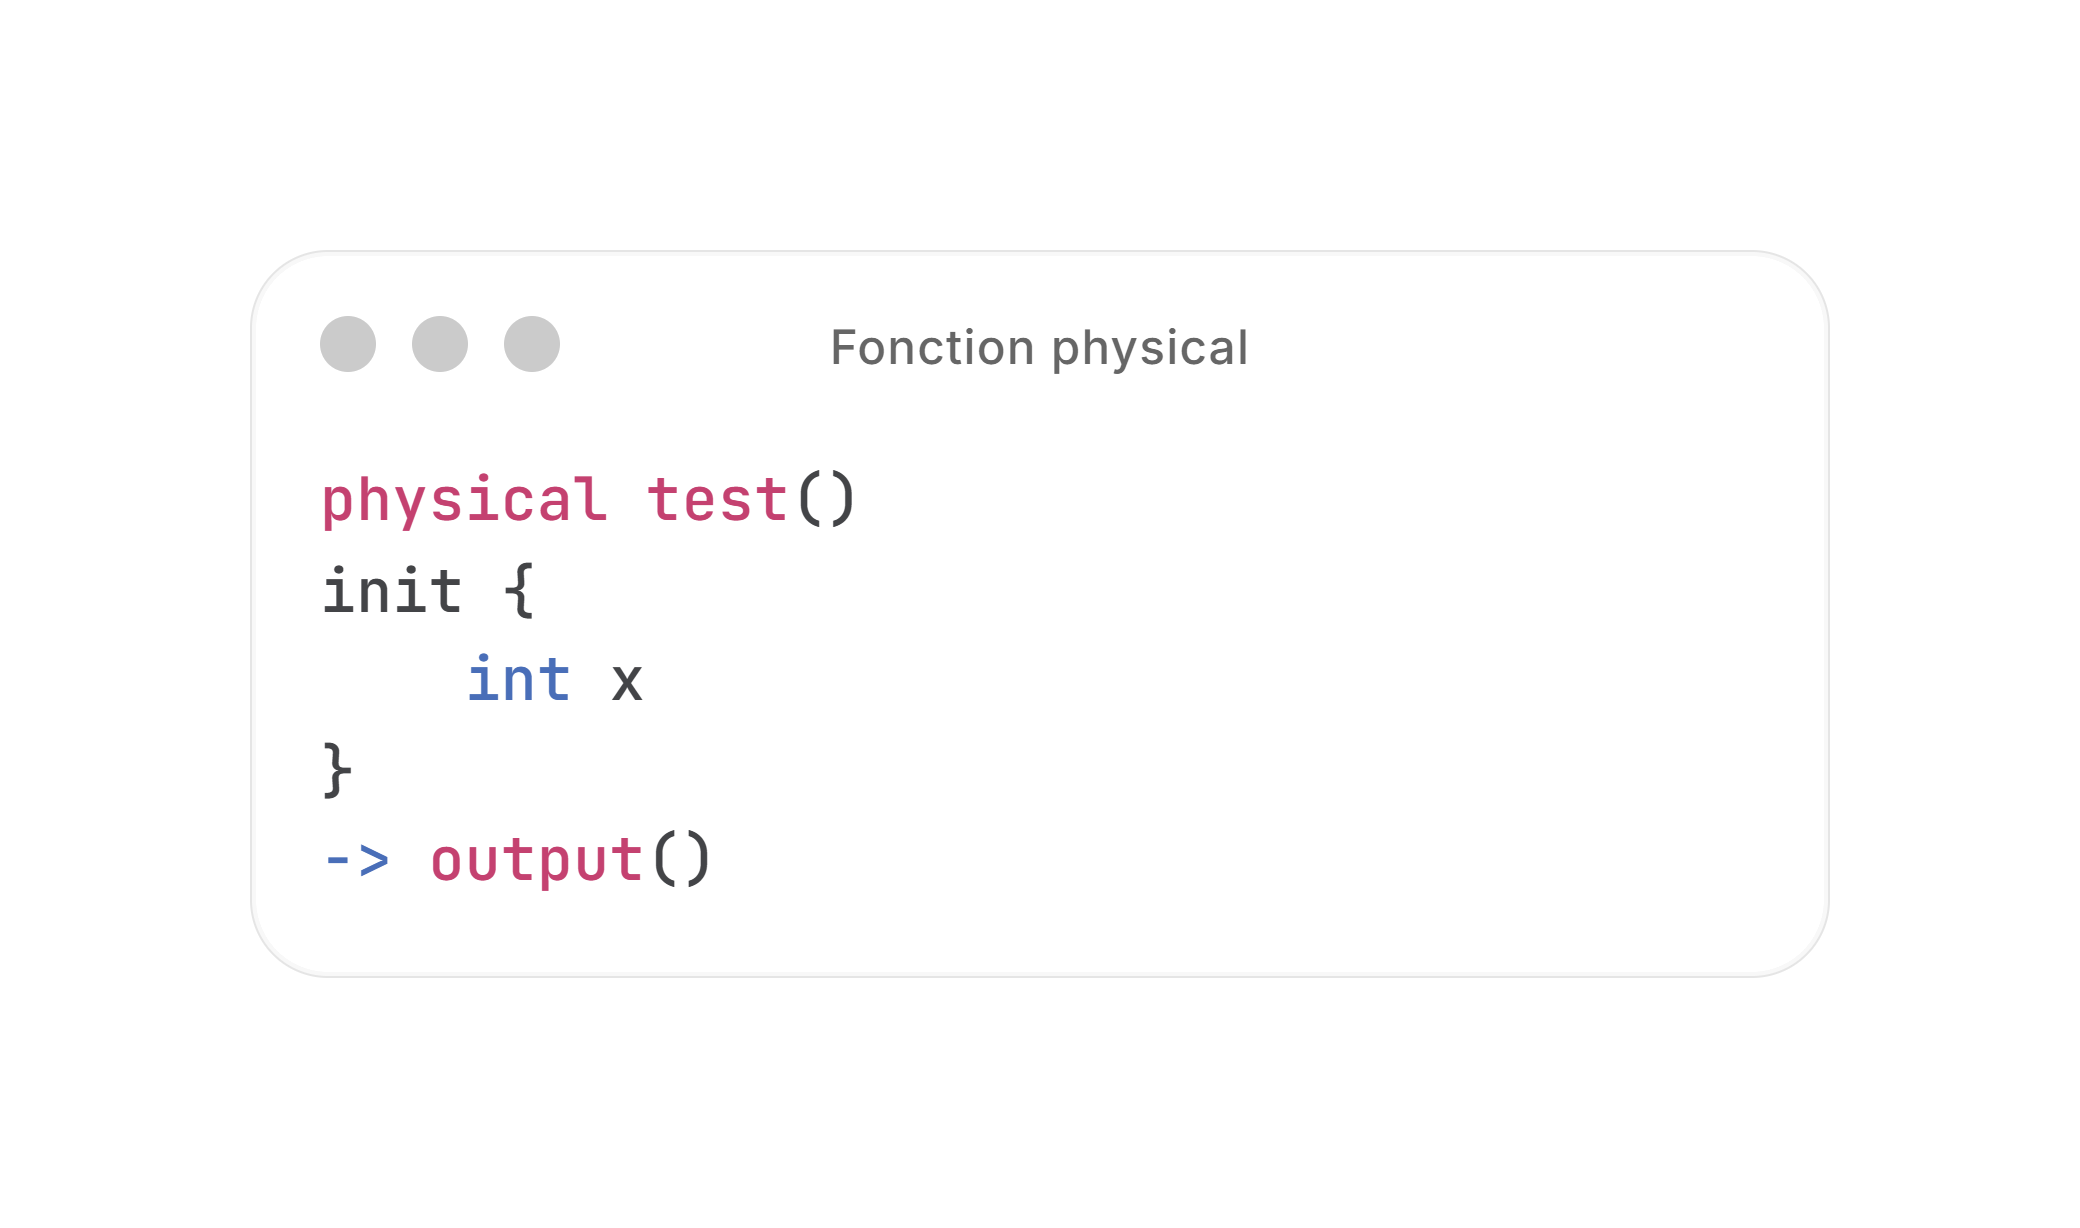
\includegraphics[width=\textwidth]{Fonction-physical.png}
    \caption{Exemple d'erreur syntaxique}
    \label{fig:erreur_syntax_physical}
\end{figure}

\begin{figure}
    \begin{itemize}
        \centering
        \item[] \prog{x = 1 + 1.0;}
    \end{itemize}
    \caption{Expression arithmétique CHIPS}
    \label{fig:expression_arithmetique}
\end{figure}

\section{Tableaux}

\begin{table}
    \centering
    \begin{tabular}{|l|l|p{5cm}|}
        \hline
        Nom de l'erreur & Exemple & Explication \\
        \hline
        TYPE\_MISMATCH & \prog{int x = 1.0} & Une variable d'un certain type ne peut recevoir des résultats d'expressions qui ne sont que de ce type.  \\
        \hline
        IMPLICIT\_CAST & \prog{1 + 1.0} & Les expressions entre 2 types différents sont complètement impossibles. \\
        \hline
        IMPLICIT\_CAST\_ASSIGNMENT & \prog{bool b = true \&\& 1 + 1.0} & Étant donné que pour la partie de droite, il n'est pas possible de calculer son type alors on sous-entend qu'il y a un cast implicite pour l'assignation alors que non. \\
        \hline
    \end{tabular}
    \caption{Erreurs sur les typages}
    \label{tab:erreur_typage}
\end{table}

\begin{table}
    \centering
    \begin{tabular}{|p{8cm}|l|p{3.5cm}|}
        \hline
        Nom de l'erreur & Exemple & Explication \\
        \hline
        UNDEFINED\_FUNCTION & \makecell{\prog{logical test() -> output()} \\ \prog{system \{ tests(); \}}}\footnote{Ce programme ne respecte pas la grammaire mais le plus important ici c'est de comprendre pourquoi elle ne fonctionne pas surtout} & Ici, on essaye d'appeler une fonction qui n'est pas définie précédemment. \\
        \hline
        DUPLICATE\_FUNCTION\_DECLARATION & \makecell{\prog{logical test() -> output()} \\ \prog{logical test() -> output2()}} & Ici on essaye de déclarer plusieurs fois une fonction portant le même nom. \\
        \hline
        WRONG\_COUNT\_OF\_ARGUMENT & \makecell{\prog{logical test() -> output()} \\ \prog{system\{ test(1); \}}} & On essaye d'appeler une fonction mais en n'incluant pas le bon nombre d'arguments. \\
        \hline
    \end{tabular}
    \caption{Erreurs sur les fonctions}
    \label{tab:erreur_fonction}
\end{table}

\begin{table}
    \centering
    \begin{tabular}{|l|l|p{5cm}|}
    \hline
        Nom de l'erreur & Exemple & Explication  \\
        \hline
         NO\_PLUGGING\_WITH\_INPUT & \makecell{\prog{logical test()-> o(1)} \\ \prog{logical test2(int x = input)} \\ \prog{system\{ test2() \}}} & Ici la fonction \prog{test2} attend d'avoir un lien au niveau de l'\prog{input} sauf qu'il n'y en a aucun. \\
         \hline
         NO\_PLUGGING\_WITH\_OUTPUT & \makecell{\prog{logical test()-> o(1)} \\ \prog{logical test2(int x = input)} \\ \prog{system\{ test.o \}}} & Ici la fonction \prog{test} attend d'avoir un lien au niveau de son \prog{output} sauf qu'il n'y en a aucun. \\
         \hline
    \end{tabular}
    \caption{Erreurs sur les fonctions pas encore gérées}
    \label{tab:erreur_fonction_non_geree}
\end{table}

\end{appendix}

\end{document}